\chapter{Architecture} 
\label{chap:architectureDesign}

The system consist of three piped object streams  (Figure: \ref{fig:tsGenArch}). Stream piping implements the idea of pipe "$|$" in Unix systems invented by Douglas Mcllroy \cite{pipe}. It enables the output of one program to be connected to the input of the next program. \textit{Object stream (Stream in an object mode)} is a stream in which a data is treated as a sequence of discrete javascript objects. The piping of object streams allows to perform parallel executions which can be beneficial from the performance perspective. 

\begin{figure}[ht]
	\label{fig:tsGenArch}
	\centering
	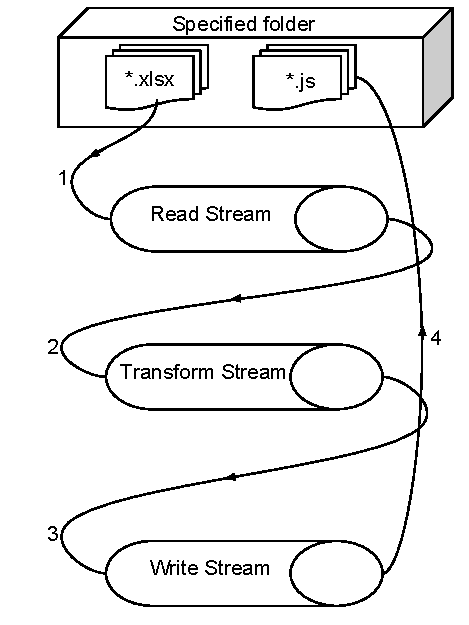
\includegraphics[scale=0.75]{grafiken/TSGeneratorArchitecture}
	\caption{Information flow}
\end{figure}

\begin{enumerate}
	\item \textbf{\textit{Read Stream}} accepts directory address and \textit{pulls} content of all spread sheet files together with their metadata  from this directory including nested directories. From this stream perspective the \textit{Transform Stream} will be referred as an \textit{up stream};
	\item \textbf{\textit{Transform Stream}} accepts the data object with the file name, content, metadata from upstream, creates TestSheet schema and generates content of javascript file implementing \textit{interpreter pattern}. From this stream perspective the \textit{Read Stream} will be referred as an \textit{down stream}, and \textit{Write Stream} as an \textit{up stream}; 
	\item \textbf{\textit{Write Stream}} \textit{pulls} data from upstream. Then is performs an attempt to read the representative .js file from the  specified folder. If the file exists and its last update date is older then for spreadsheet file then the next step will be skipped. If the file does not exist or its the last update date is earlier then the last update date of spreadsheet file then it creates/overwrites javascript file. From this stream perspective the \textit{Transform Stream} will be referred as an \textit{down stream};
\end{enumerate}

Pipe method of streams provide developers with an opportunity to chain streams implementing different piping patterns:
\begin{enumerate}
	\item \textit{Combining} - encapsulation of sequentualy connected streams in to single looking stream with single I/O points and single error handling mechanism by pipeing readable stream in to writable stream;
	\item \textit{Forking/Merging} - piping single readable in to multiple writable streams /  piping multiple readable streams in to single writable stream;
	\item \textit{Multiplexing/Demultiplexing} - forking and merging pattern which provides shared communication channel for entities from different streams, analogy can be computer networks.
\end{enumerate}

As was already described streams are deferred analog of arrays, which allows to perform such operations as mapping, reducing and filtering. The process of transformation of xlsx files to js files in this application is treated as mapping process in general case, and filtering for avoiding of redundant file's overwriting in case if a source xlsx file was not updated.

The folder/file structure of the application looks as following:
\begin{itemize}
	\item index.js
	\item package.json
	\item ReadMe.md
	\item lib/
	\begin{itemize}
		\item scheme/
		\begin{itemize}
			\item index.js
			\item execution\_scheme.js
			\item order.js
			\item scheme.js
		\end{itemize}
		\item stream/
		\begin{itemize}
			\item index.js
			\item read\_stream.js
			\item transform\_stream.js
			\item write\_stream.js
		\end{itemize}
		\item template/
		\begin{itemize}
			\item index.js
		\end{itemize}
	\end{itemize}
	\item test/
	\begin{itemize}
		\item read\_stream.js
		\item write\_stream.js
		\item transform\_stream.js
		\item scheme.js
		\item execution\_scheme.js
		\item order.js
		\item template.js
		\item doublers/
		\begin{itemize}
			\item TestSheetOjbect.js
			\item TestSheet.xlsx
			\item TestSheet.js
		\end{itemize}
	\end{itemize}
	\item node\_modules/
\end{itemize}
%Creation of folders for scheme and template directories is made for purpose of expansion in case of adding Non-linear and/or HigherOrder Test Sheets. 
The entry point of the system ./index.js looks as following (Listing: \ref{index}):

\lstinputlisting[
language=Javascript, numbers=left, stepnumber=5, firstnumber=1, breaklines=true, 
basicstyle=\footnotesize,
numberstyle=\tiny,
caption={index.js},
captionpos=b,
label=index
]
{code/index.js.txt}

The program invoked from the command line interface accepts one parameter - path to the folder with xlsx files which stores Test Sheets defined by users. The \textit{argv} property of \textit{process} is an array of parameters with which the node module was called from a command line interface. The first parameter is a module name. All next parameters are the arguments passed to this module.

Each directory unifies node modules for implementation of representative logic. Every folder has \textit{index.js} file which is the public interface file of the module. The default behavior of the \textit{require} method from node.js is to require the \textit{index.js} file from folder if path to it is passed as an input parameter, and file if an input parameter is a path to the file.

